\section{Nutzerstudien}
Wie bereits in der Beschreibung des Qualitätsziels Bedienbarkeit (Abschnitt \ref{bedienbarkeit_qs})
erwähnt, wurden während des Projekts zwei Nutzerstudien durchgeführt. Diese wurde sowohl mit
Mitarbeitern des Fachgebiets als auch mit Studierenden aus anderen Fachbereichen durchgeführt.
Dadurch wurde getestet, ob die Oberfläche sowohl für Personen mit Flugsimulatorefahrung, als auch
von Laien bedienbar ist.
\\\\
Beide Nutzerstudien hatten jeweils einen anderen Fokus:
Die erste Studie konzentrierte sich auf das Aufsetzen der Software, während in der zweiten Studie
die Ablaufprogrammierung von Startsequenzen im Mittelpunkt stand. Daher ergaben sich zwei unterschiedliche
Fragebögen.
\\\\
Eine Zusammenfassung der Ergebnisse findet sich jeweils nach dem Fragebogen.

\subsection{Nutzerstudie 1}
Die erste Studie hatte das Ziel zu testen, ob die vorgesehenen Arbeitsabläufe für die Nutzer
intuitiv durchführbar waren. Zudem wurde zum ersten Mal die Oberfläche der Software Mitarbeitenden und Studierenden
vorgeführt, welche nicht Teil des BP-Teams bzw. Auftraggebern waren. Sie fand am 12.02.2018 statt.
\includepdf[pages={1-},scale=0.9]{../Nutzerstudie/Studie1/Aufgaben.pdf}
\includepdf[pages={1-},scale=0.9]{../Nutzerstudie/Studie1/fragebogen.pdf}
\subsubsection{Ergebnisse}
Viele Teilnehmenden an der Studie wünschten sich kleinere Designänderungen, beispielsweise die Vergrößerung von
Buttons oder ähnliche kleinere Veränderungen an der Oberfläche. Dies wurden vom Team während einer Refactoring-Phase
eingearbeitet. Die sonstigen Maßnahmen wurden in Absprache mit den Auftraggebern zu Userstorys umgewandelt und
in der nächsten Iteration fertiggestellt. Die Zuweisung findet sich in Tabelle \ref{studie1_us}
\\\\
{\large Feedback der Nutzer\\}
\begin{enumerate}
\item Allgemein
\begin{enumerate}
	\item Alle Slaves in Clients umbenennen (gefunden in den Skripten)
	\item Übersichtsseite mit allen Events, nach Clients sortiert
	\item Tooltips für alle Felder
	\item Pluszeichen zu klein/alternatives Symbol oder Satz verwenden
	\item (Event-)Log-Dateien
	\item Inputhints
	\item Dateien und Programme über Clientgrenzen kopieren
	\item Abtrennung zwischen den Feldern verstärken
	\item Breiter Statusbalken
	\item Home Button
	\item Mehr Bilder/Icons
\end{enumerate}
\item Anlegen eines Programms
\begin{enumerate}
	\item Startzeit ist nicht erklärt, Wert -1 verwirrt
	\item Dateisystembrowser
\end{enumerate}
\item Anlegen eines Clients
\begin{enumerate}
	\item Nach Anlegen eines Clients soll dieser automatisch ausgewählt werden
	\item Verfügbare IP/MAC-Adressen anzeigen
	\item Beschreibungstext
\end{enumerate}
\item Anlegen einer Datei
\begin{enumerate}
	\item Anzeigename in Name umbennen
\end{enumerate}
\item Anlegen eines Scripts
\begin{enumerate}
	\item Nachfrage bevor Tab/Browser geschlossen wird
	\item alternativ autosave
	\item Apply statt edit
\end{enumerate}
\item Run Script
\begin{enumerate}
	\item Run Knopf hervorheben
	\item Reload nach Klick auf 'Run Script'
	\item Gesamtprozess in Skript anzeigen
\end{enumerate}
\item Delete Fenster
\begin{enumerate}
	\item Statt OK explizit delete schreiben
\end{enumerate}
\end{enumerate}

\begin{table}[H]
	\centering
	\begin{tabular}{c|c}
		Anmerkung & Userstory \\\hline
		1.c & 45\\
		1.e & 37\\
		2.a & 45\\
		3.c & 45\\
		5.a & 40\\
		5.c & 37\\
	\end{tabular}
	\caption{Zuordnung von Anmerkung zu Userstory}
	\label{studie1_us}
\end{table}

\subsubsection{Ausgefüllte Bögen}
\begin{center}
	\includepdf[pages=1-,width=.9\textwidth]{nutzerstudie1}
\end{center}

\subsection{Nutzerstudie 2}
Das Ziel dieser Studie war das Feintuning der Oberfläche und das Testen des neuen
Skripteditors. Die Studie fand am 12.03.2018 statt. Die Studie wurde durchgeführt,
obwohl das Projekt bereits kurz vor Ende stand, da die Auftraggeber eine
Weiterentwicklung wünschten und die Ergebnisse an das nachfolgende Entwickler
weitergegeben werden.
\includepdf{../Nutzerstudie/Studie2/Aufgaben.pdf}
\includepdf{../Nutzerstudie/Studie2/fragebogen.pdf}
\subsubsection{Ergebnisse}
Diese Studie ergab sehr wenig Feedback, da alle Anmerkungen der ersten Studie bereits
eingearbeitet wurden. Die Designänderungen wurden wie in der ersten Nutzerstudie
vom Team eingearbeitet. Die Zuweisung zu den passenden Userstorys existiert hier nicht,
da sich keine Userstorys aus dieser Studie ergeben haben.
\\\\
{\large Feedback der Nutzer\\}
\begin{enumerate}
\item Interface
\begin{enumerate}
	\item Reset Filesystem in Restore Filesystem umbenennen.
	\item Deutsche Übersetzung
	\item INDEX bei Skripterstellung durch einfacheren Begriff ersetzen (Starting order)
	\item Namensgebung insgesamt überarbeiten
	\item Bei fehlerhaften Pfaden bleibt der Log leer
	\item Gestoppte Programme irgendwann zurücksetzen bzw. roter Statusbalken entfernen
	\item Kurzanleitungen innerhalb der Oberfläche anzeigen
\end{enumerate}
\item Run
\begin{enumerate}
	\item Nur anzeigen, wenn Skript läuft und in Running oder Running Script umbennen
\end{enumerate}
\item Program
\begin{enumerate}
	\item Bei Arguments vermerken, dass \textbackslash\textbackslash statt \textbackslash verwendet werden muss.
	\item Zeigt den Status vom Datenpool überall an/Benachrichtigung über Programmabsturz
	\item Übersicht aller laufenden Programme
\end{enumerate}
\item Forms
\begin{enumerate}
		\item Felder sind teilweise zu groß (Programpfad), wodurch die Form größer als ein Bildschirm ist
\end{enumerate}
\end{enumerate}
\subsubsection{Ausgefüllte Bögen}
\begin{center}
	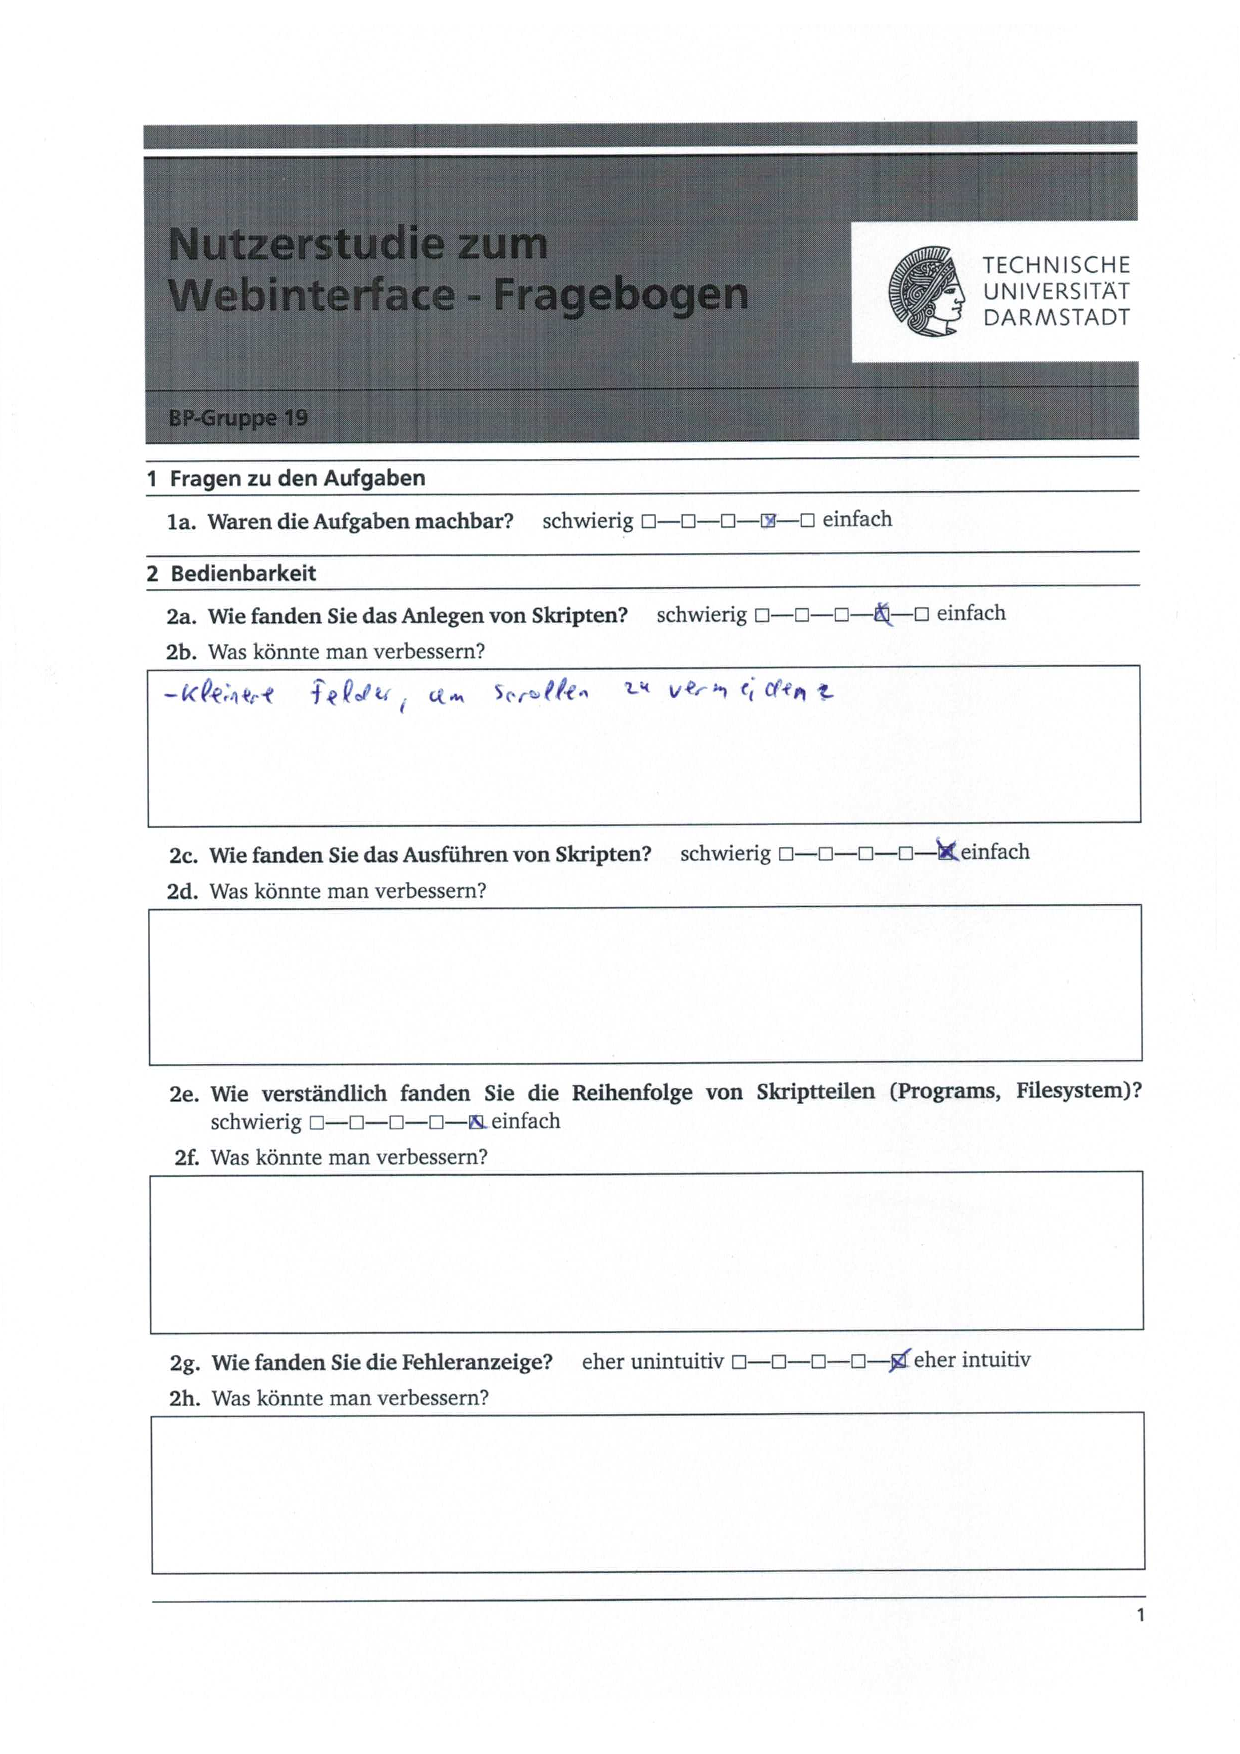
\includepdf[pages=1-,width=.9\textwidth]{nutzerstudie2}
\end{center}
